% ================================================================
% CHAPTER 3: Domänenanalyse: Domänenmodell
% ================================================================

\section{Bildmaterial aus ersten Tests}

In der Nacht vom 31. März 2020 auf den 1. April 2020 ist auf dem Betrieb vom Auftraggeber Peter Müller ein Kalb geboren. Das Bildmaterial zur Geburt zeigt einige Geburtsanzeichen, welche Merkmale aus der Literaturrecherche und aus Interviews beispielhaft veranschaulichen. Zudem ist auf den Bildern gemäss Aussage von \citep{Muller2020a} klar erkennbar, wie die Klauen des Kalbes aus der Kuh austreten. Diese Erkenntnis ergänzt das Wissen aus der der bisherigen Domänenanalyse. Folgend die wichtigsten Ergebnisse von der Klassifikation der Kamerabilder. \\





\begin{figure}[h]
	\center
	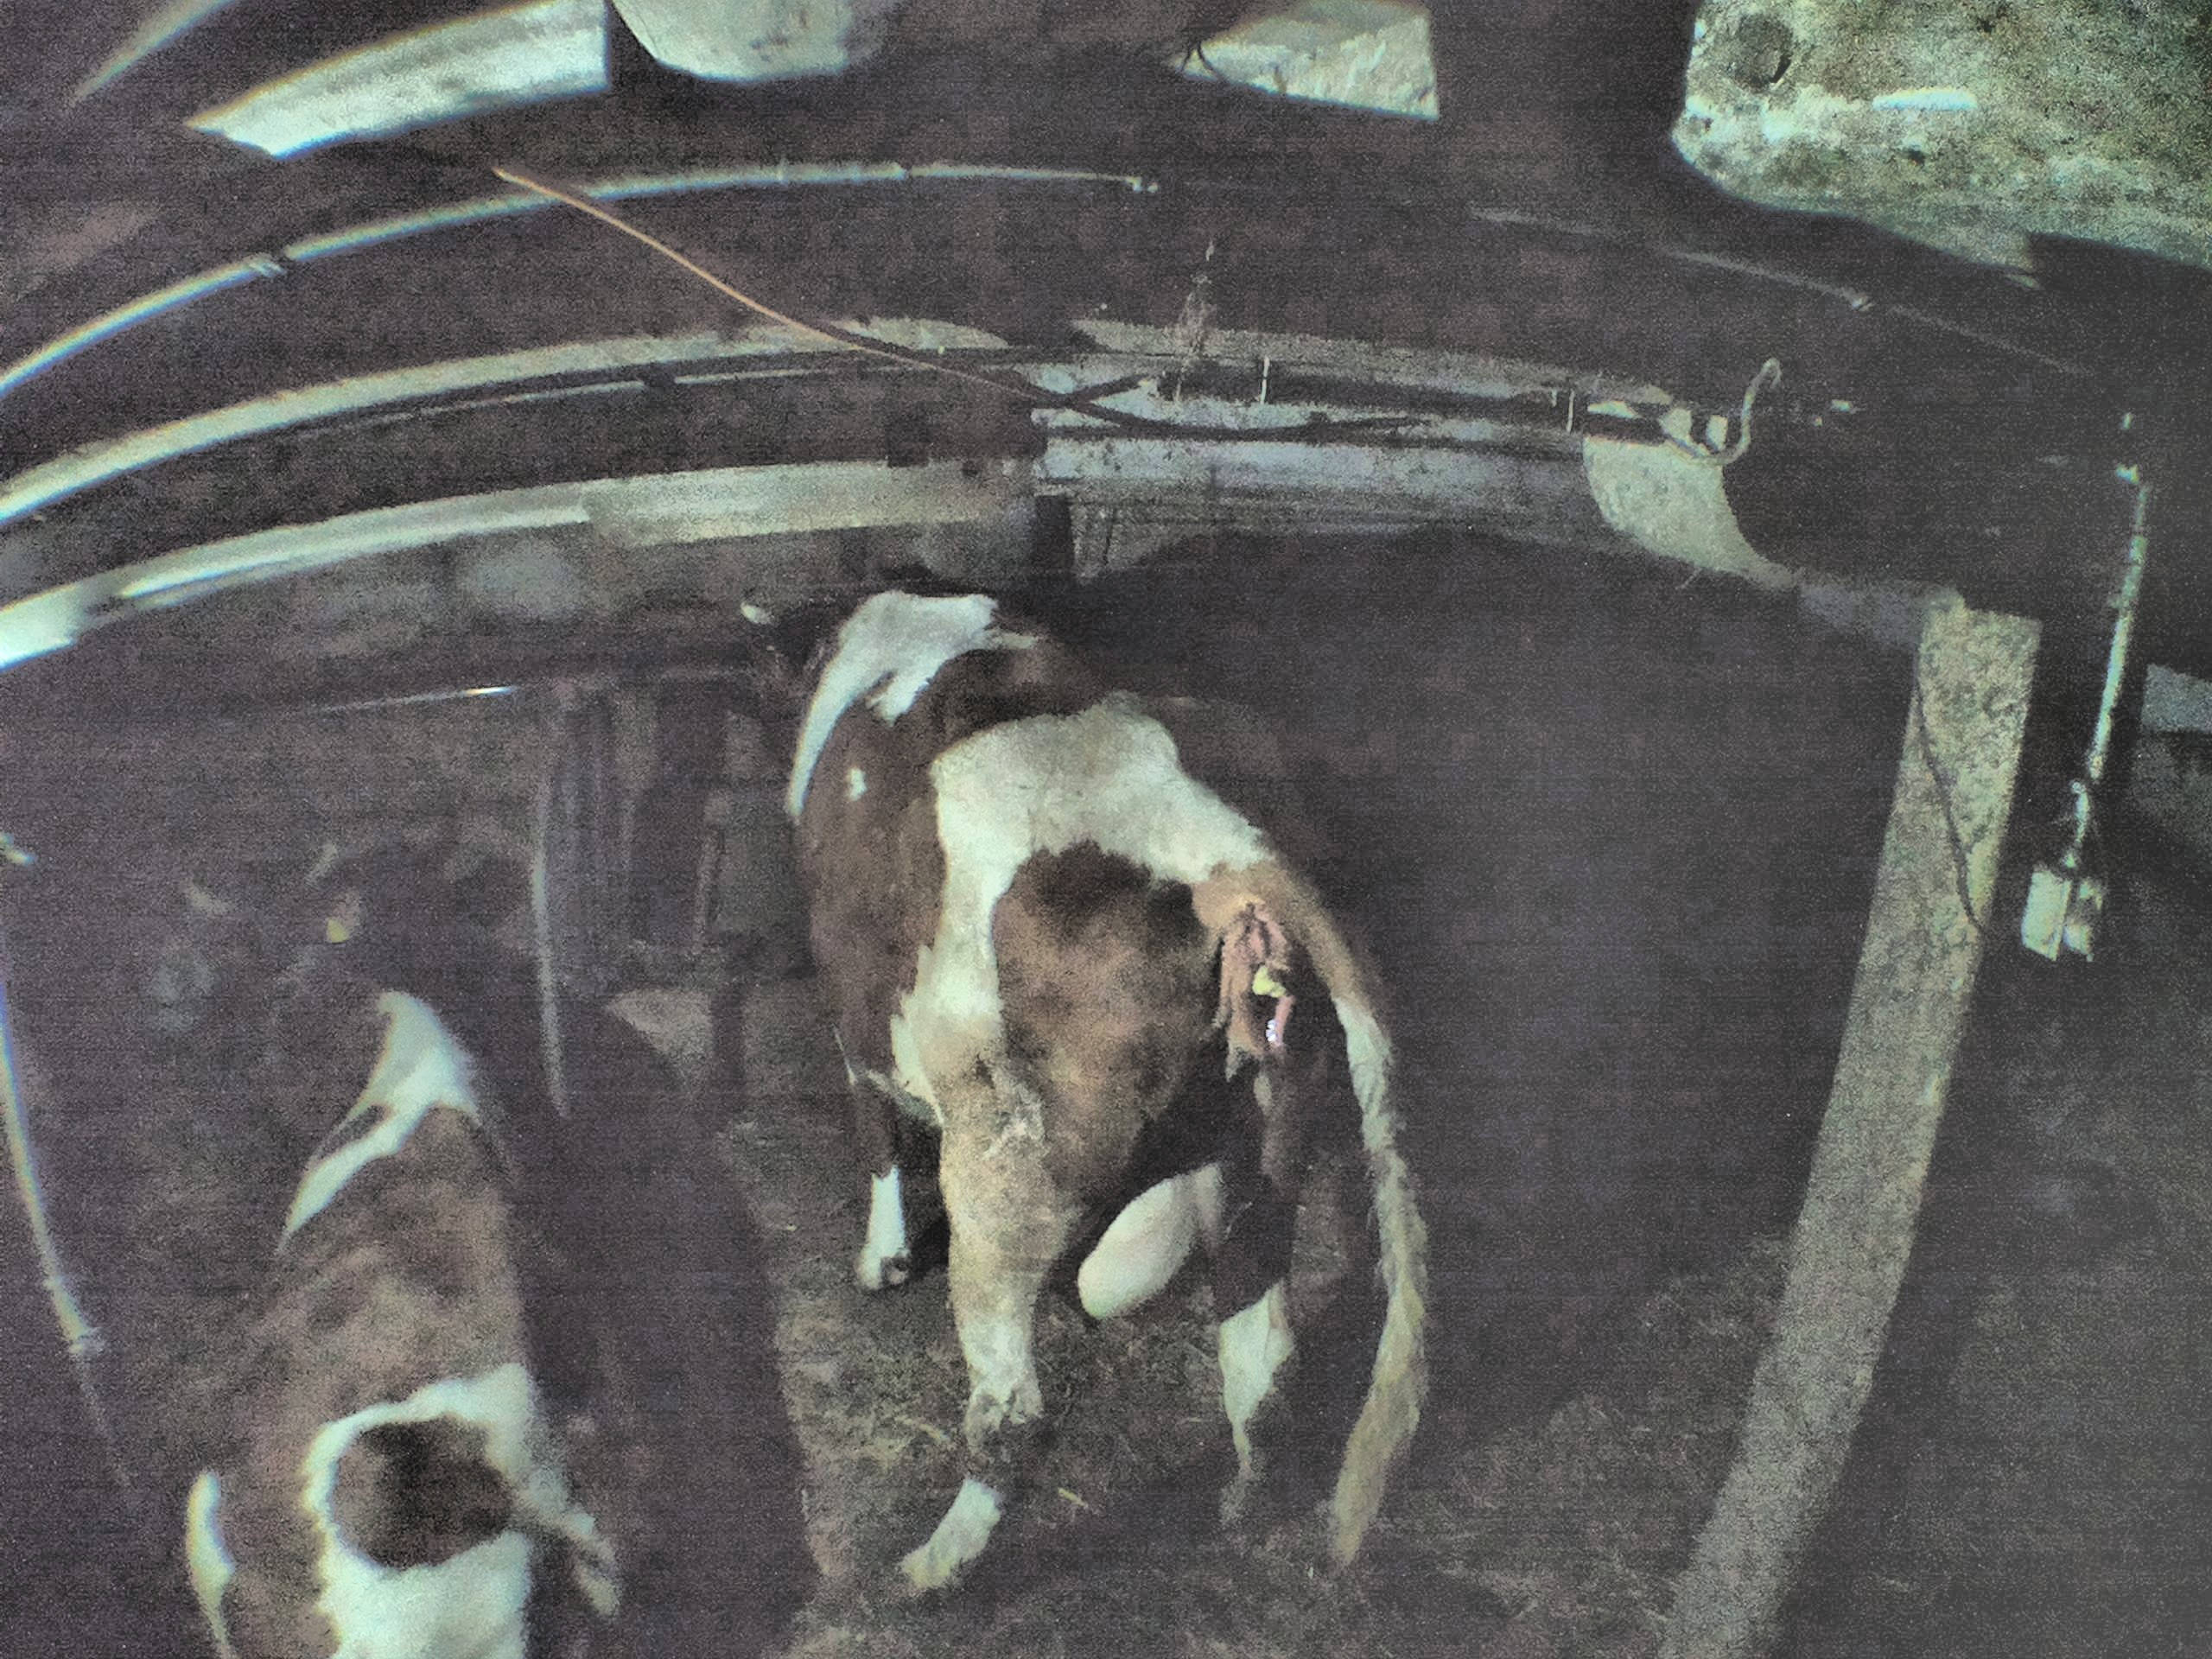
\includegraphics[scale=0.075]{Grafiken/austrittklauen.jpg}
	\caption{Austritt der Klauen des Kalbes \citep{Muller2020a}} 
	\label{fig: Austritt der Klauen des Kalbes}
\end{figure}


\begin{figure}[h]
	\center
	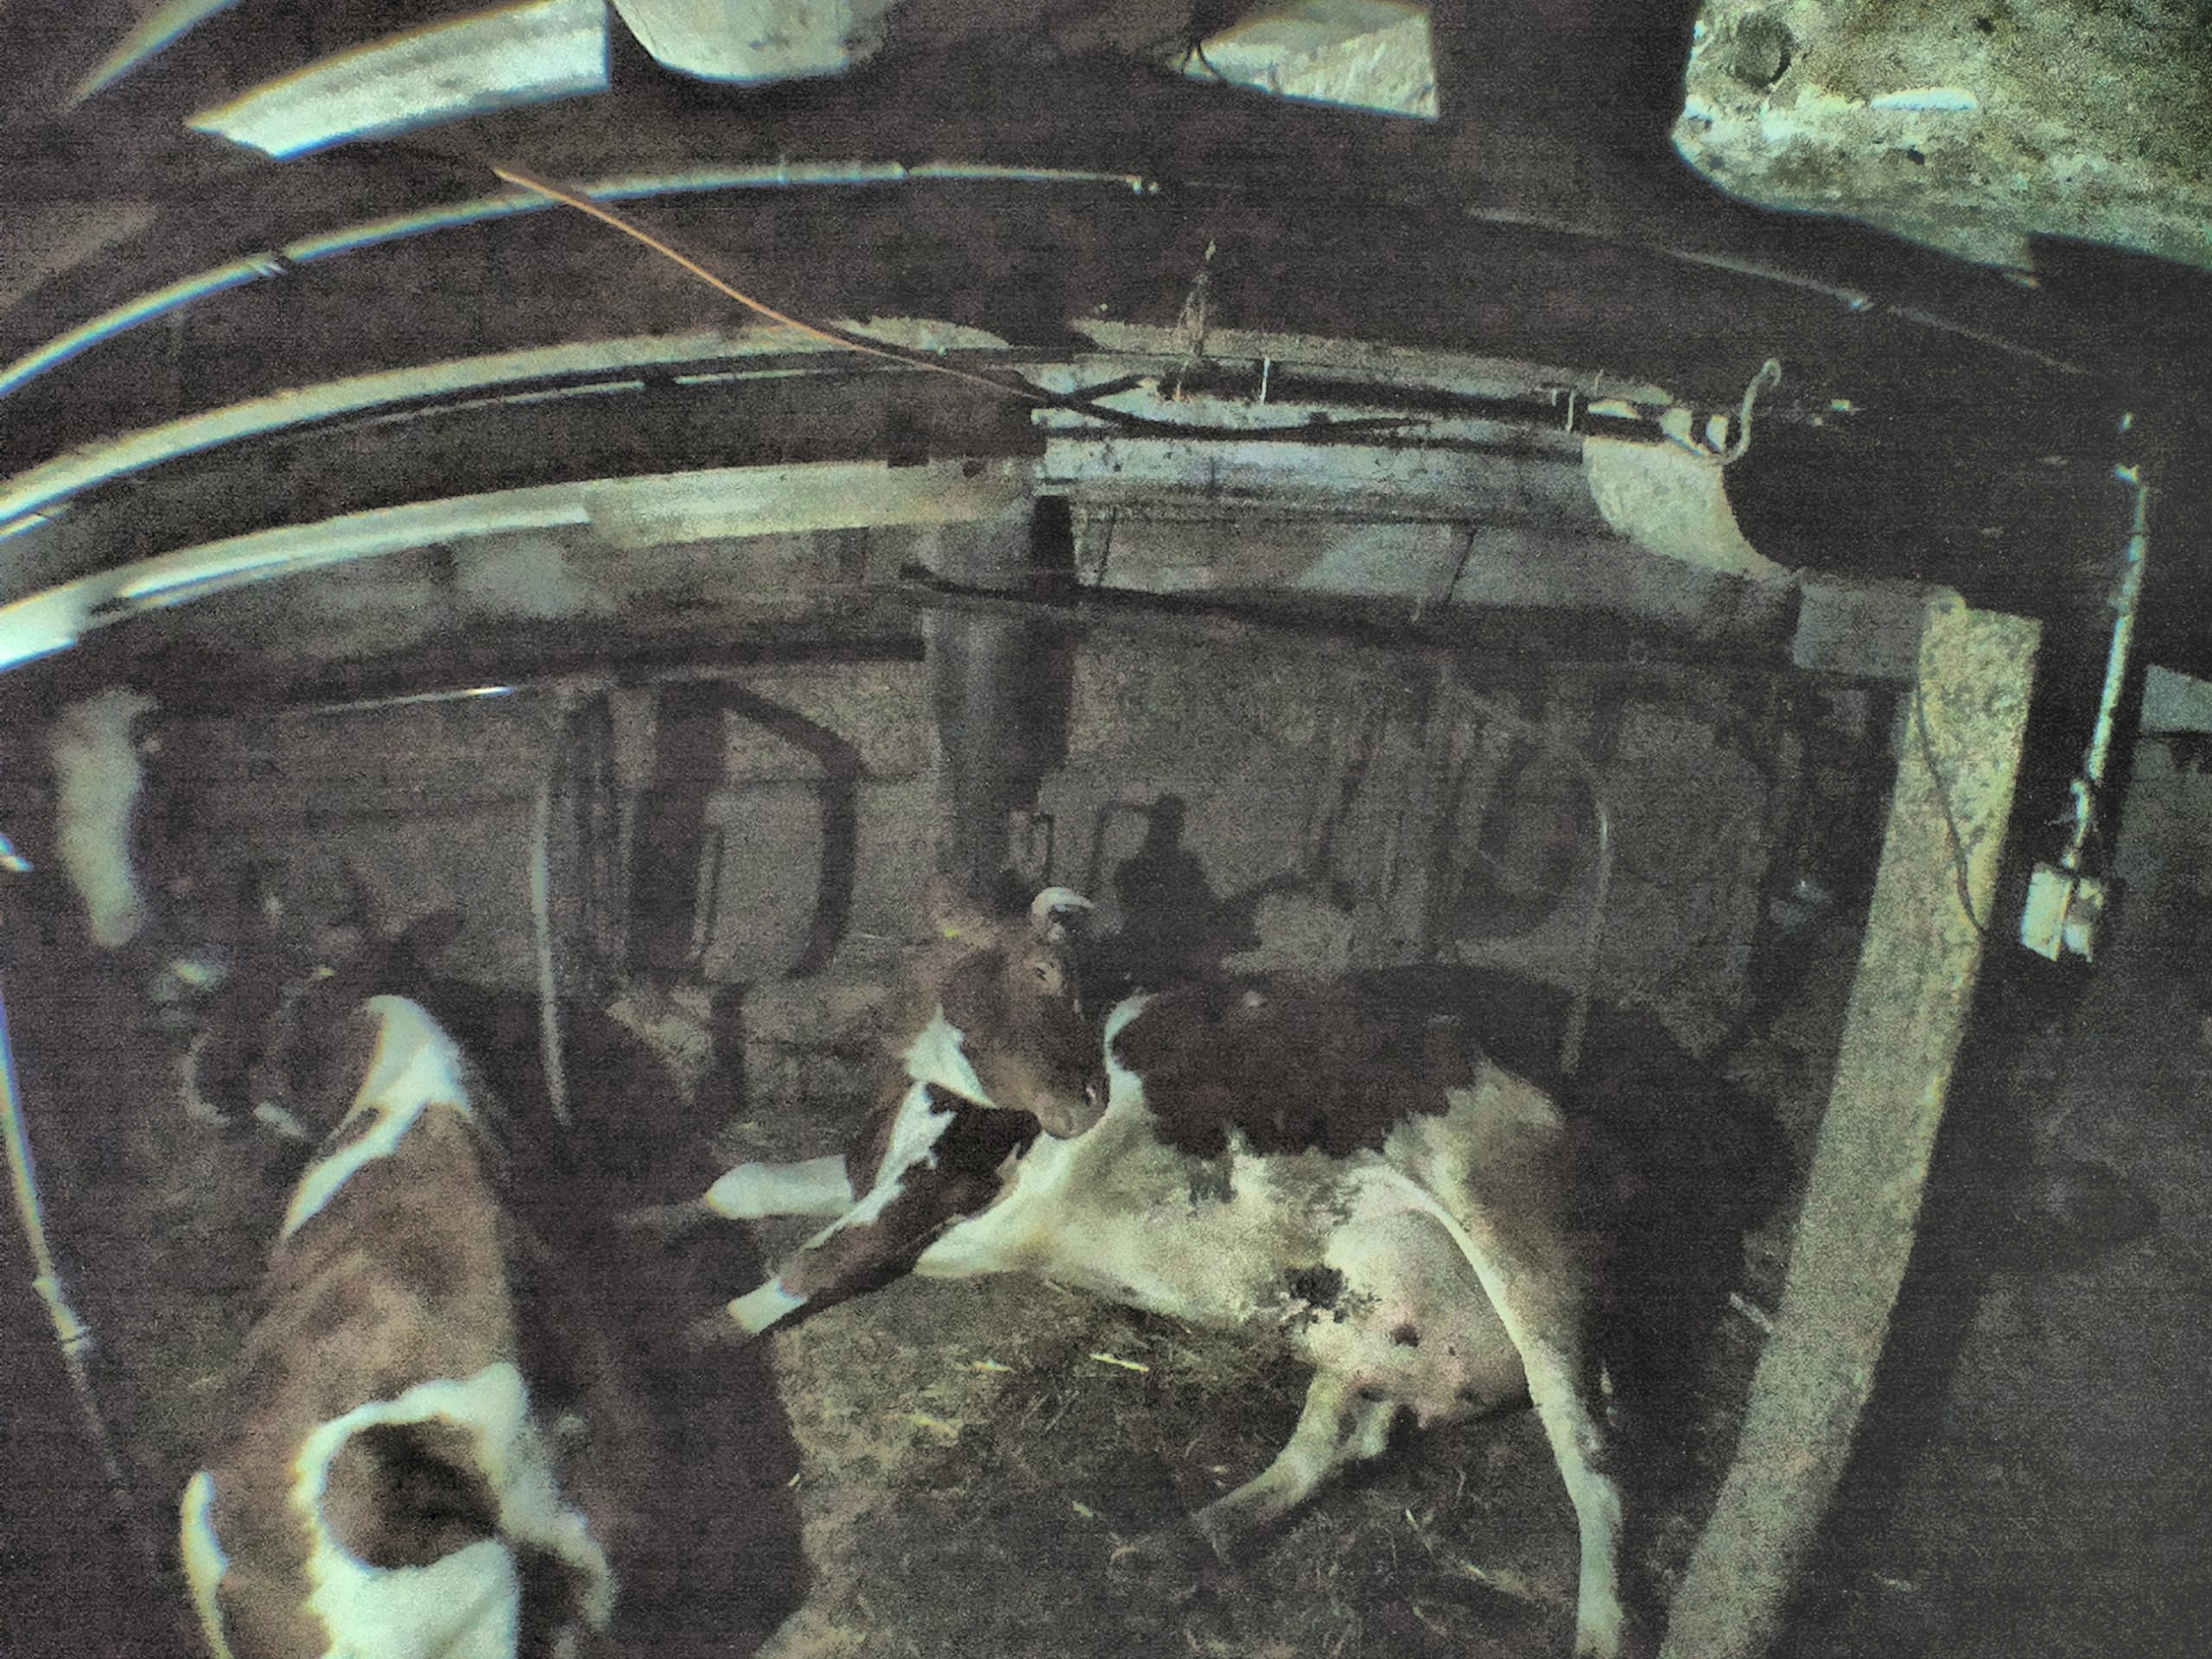
\includegraphics[scale=0.075]{Grafiken/seitlichesligen.jpg}
	\caption{Seitliches Liegen kurz vor der Geburt des Kalbes} 
	\label{fig: Seitliches Liegen kurz vor der Geburt des Kalbes}
\end{figure}


\begin{figure}[h]
	\center
	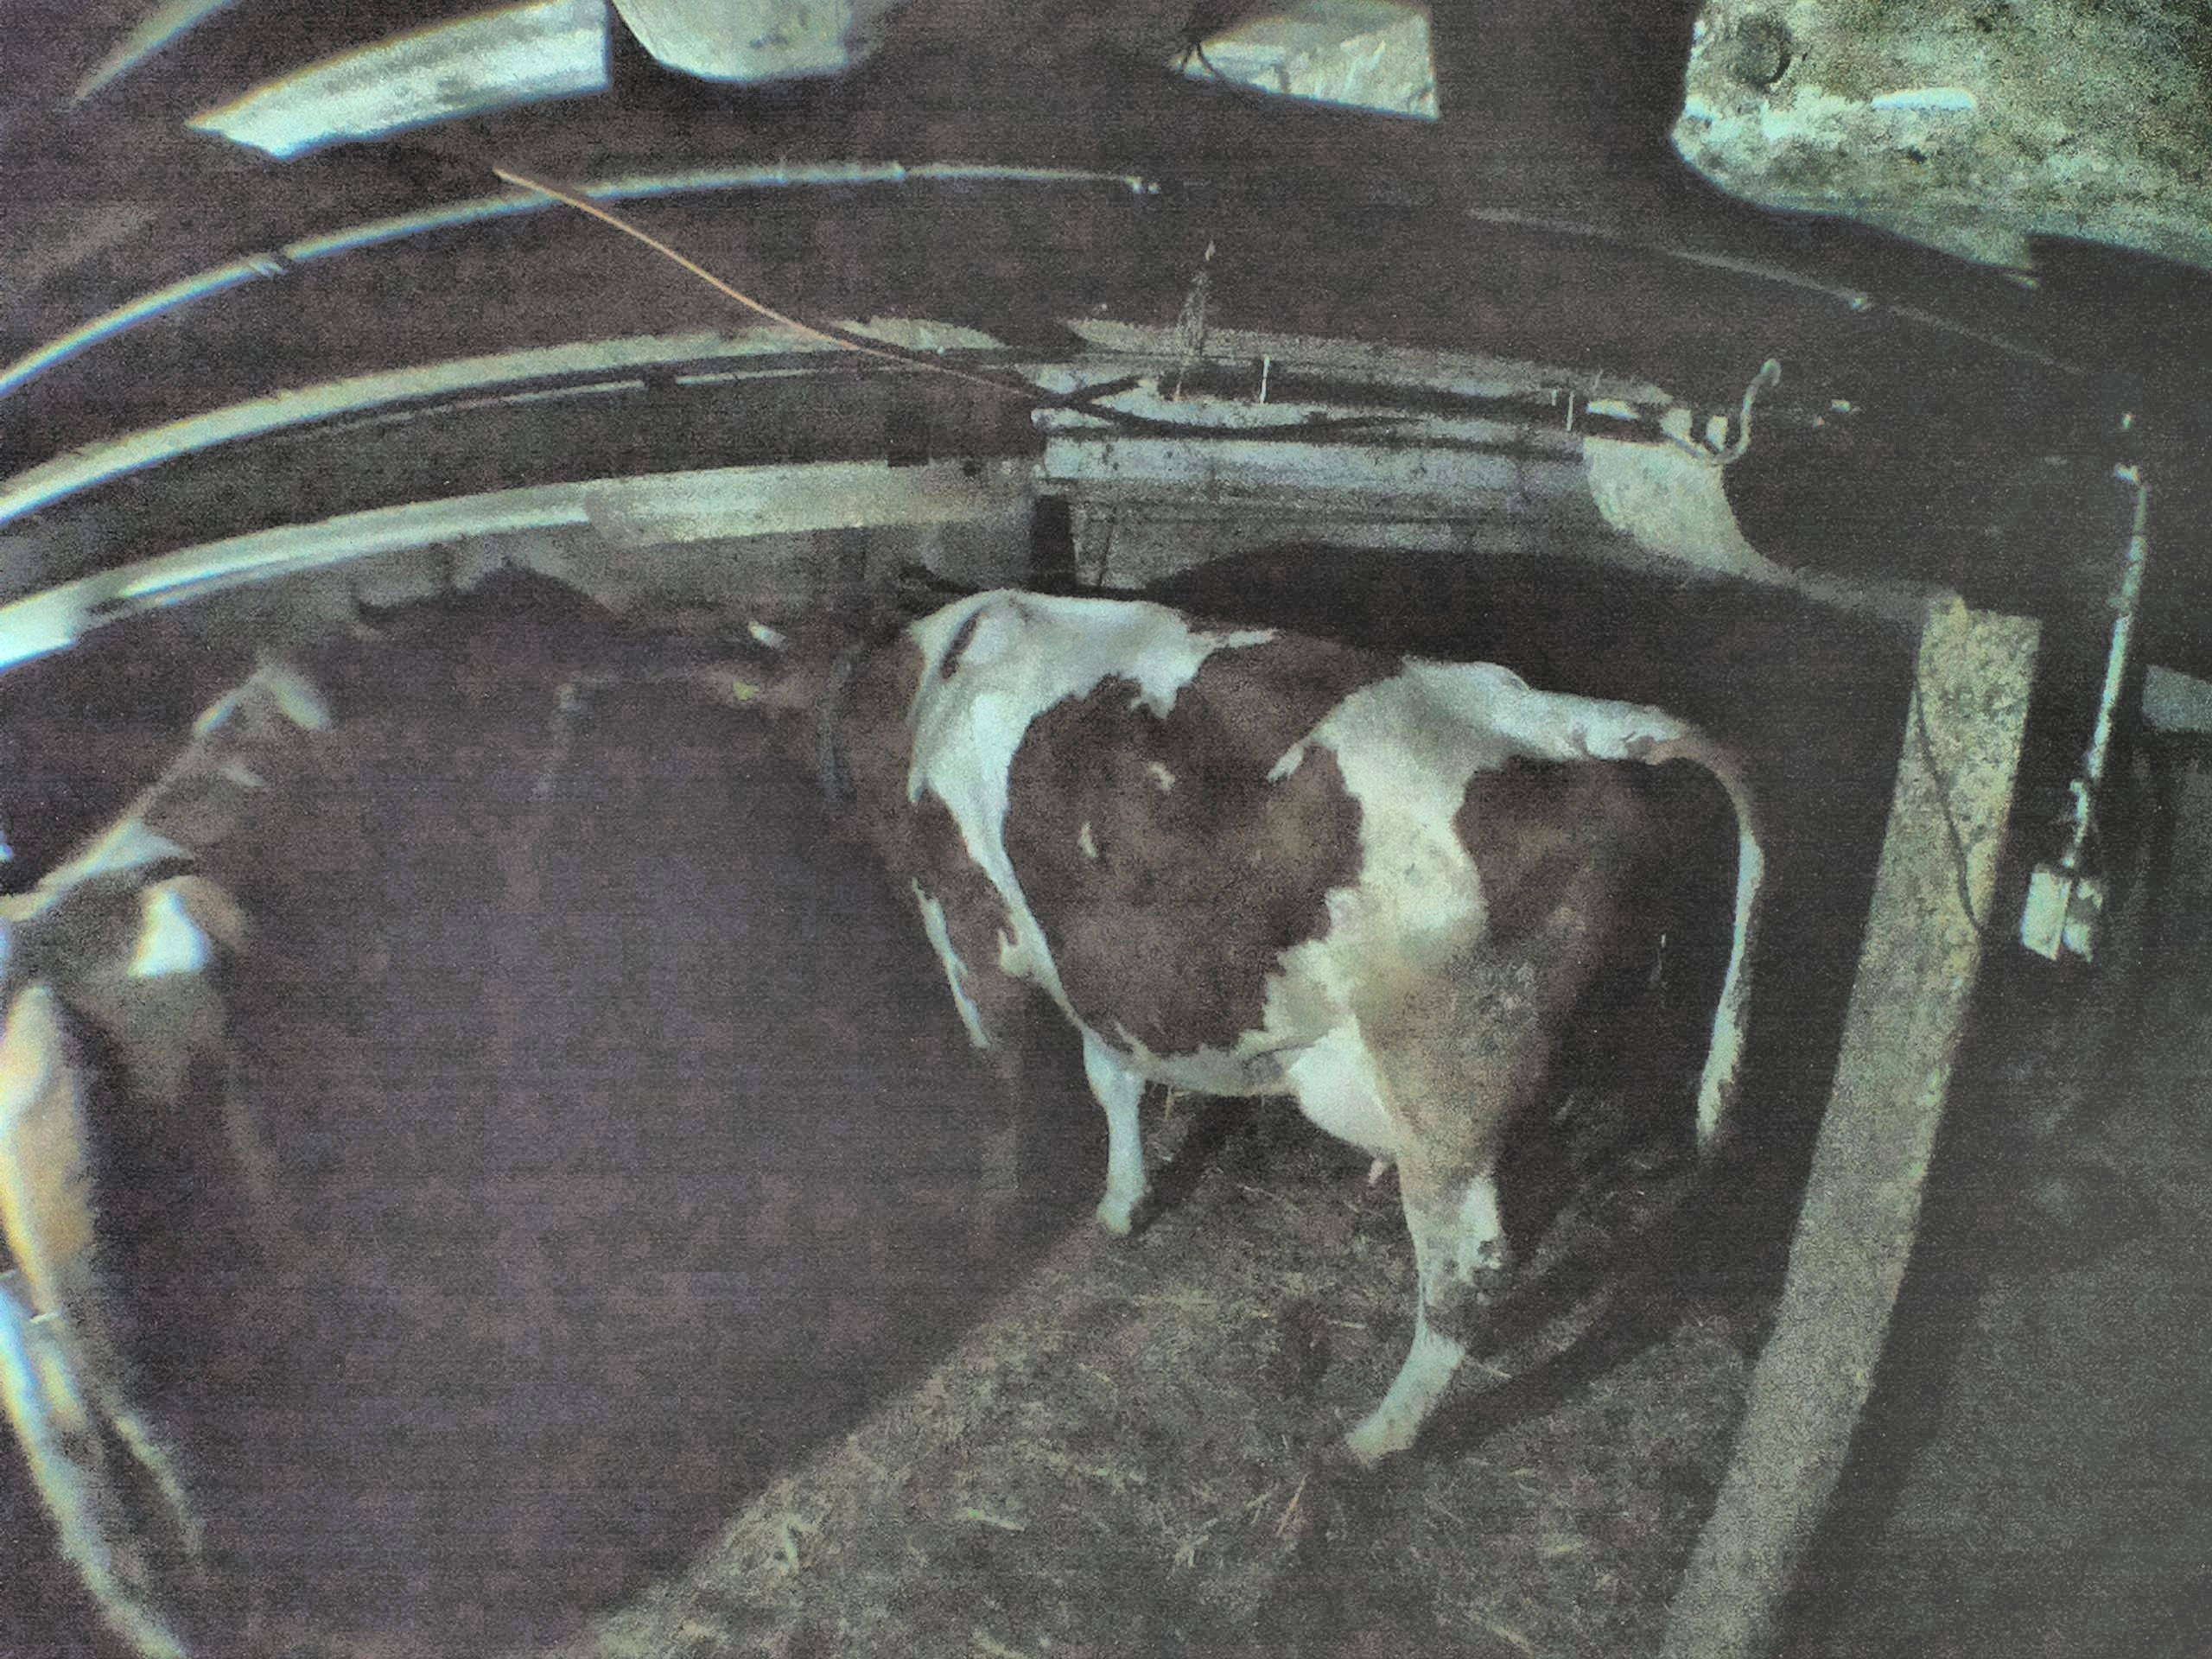
\includegraphics[scale=0.075]{Grafiken/schwanhebungkamerabild.jpg}
	\caption{Kamerabild der Schwanzhebung} 
	\label{fig: Kamerabild der Schwanzhebung}
\end{figure}

\begin{figure}[h]
	\center
	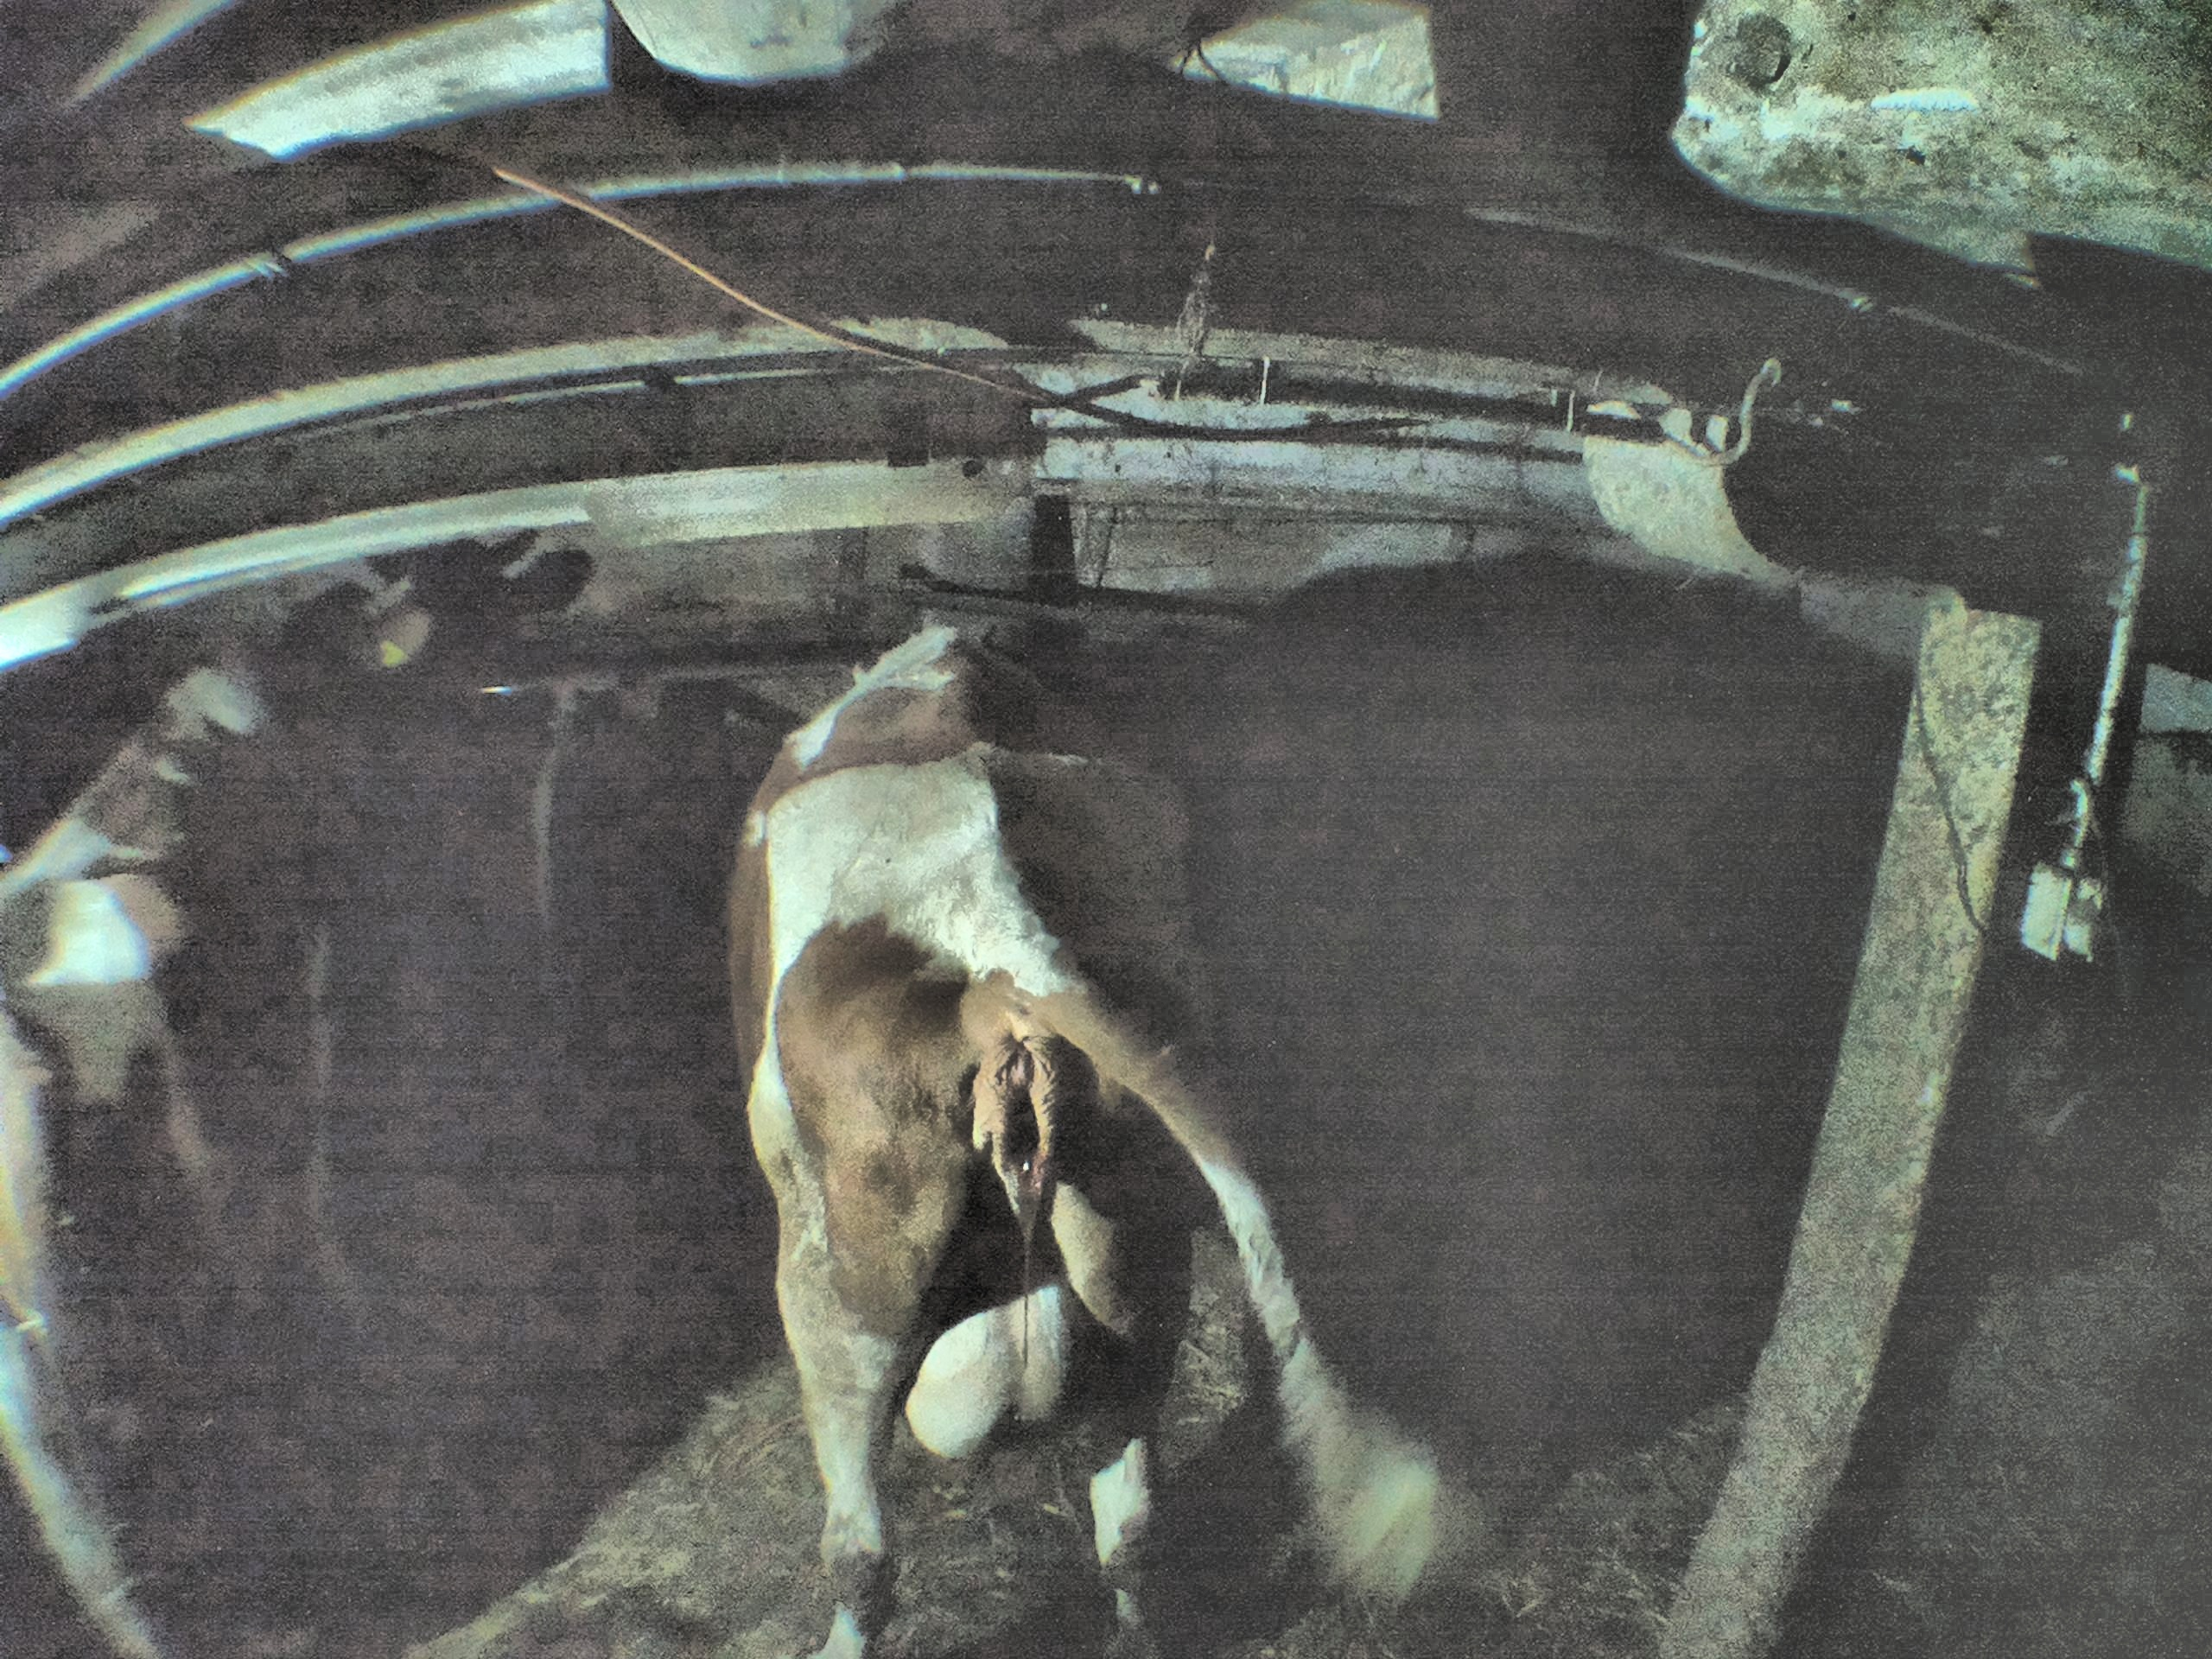
\includegraphics[scale=0.075]{Grafiken/schleimvagina.jpg}
	\caption{Schleim im Schambereich der Kuh kurz vor der Geburt} 
	\label{fig: Schleim im Schambereich der Kuh kurz vor der Geburt}
\end{figure}


\begin{figure}[h]
	\center
	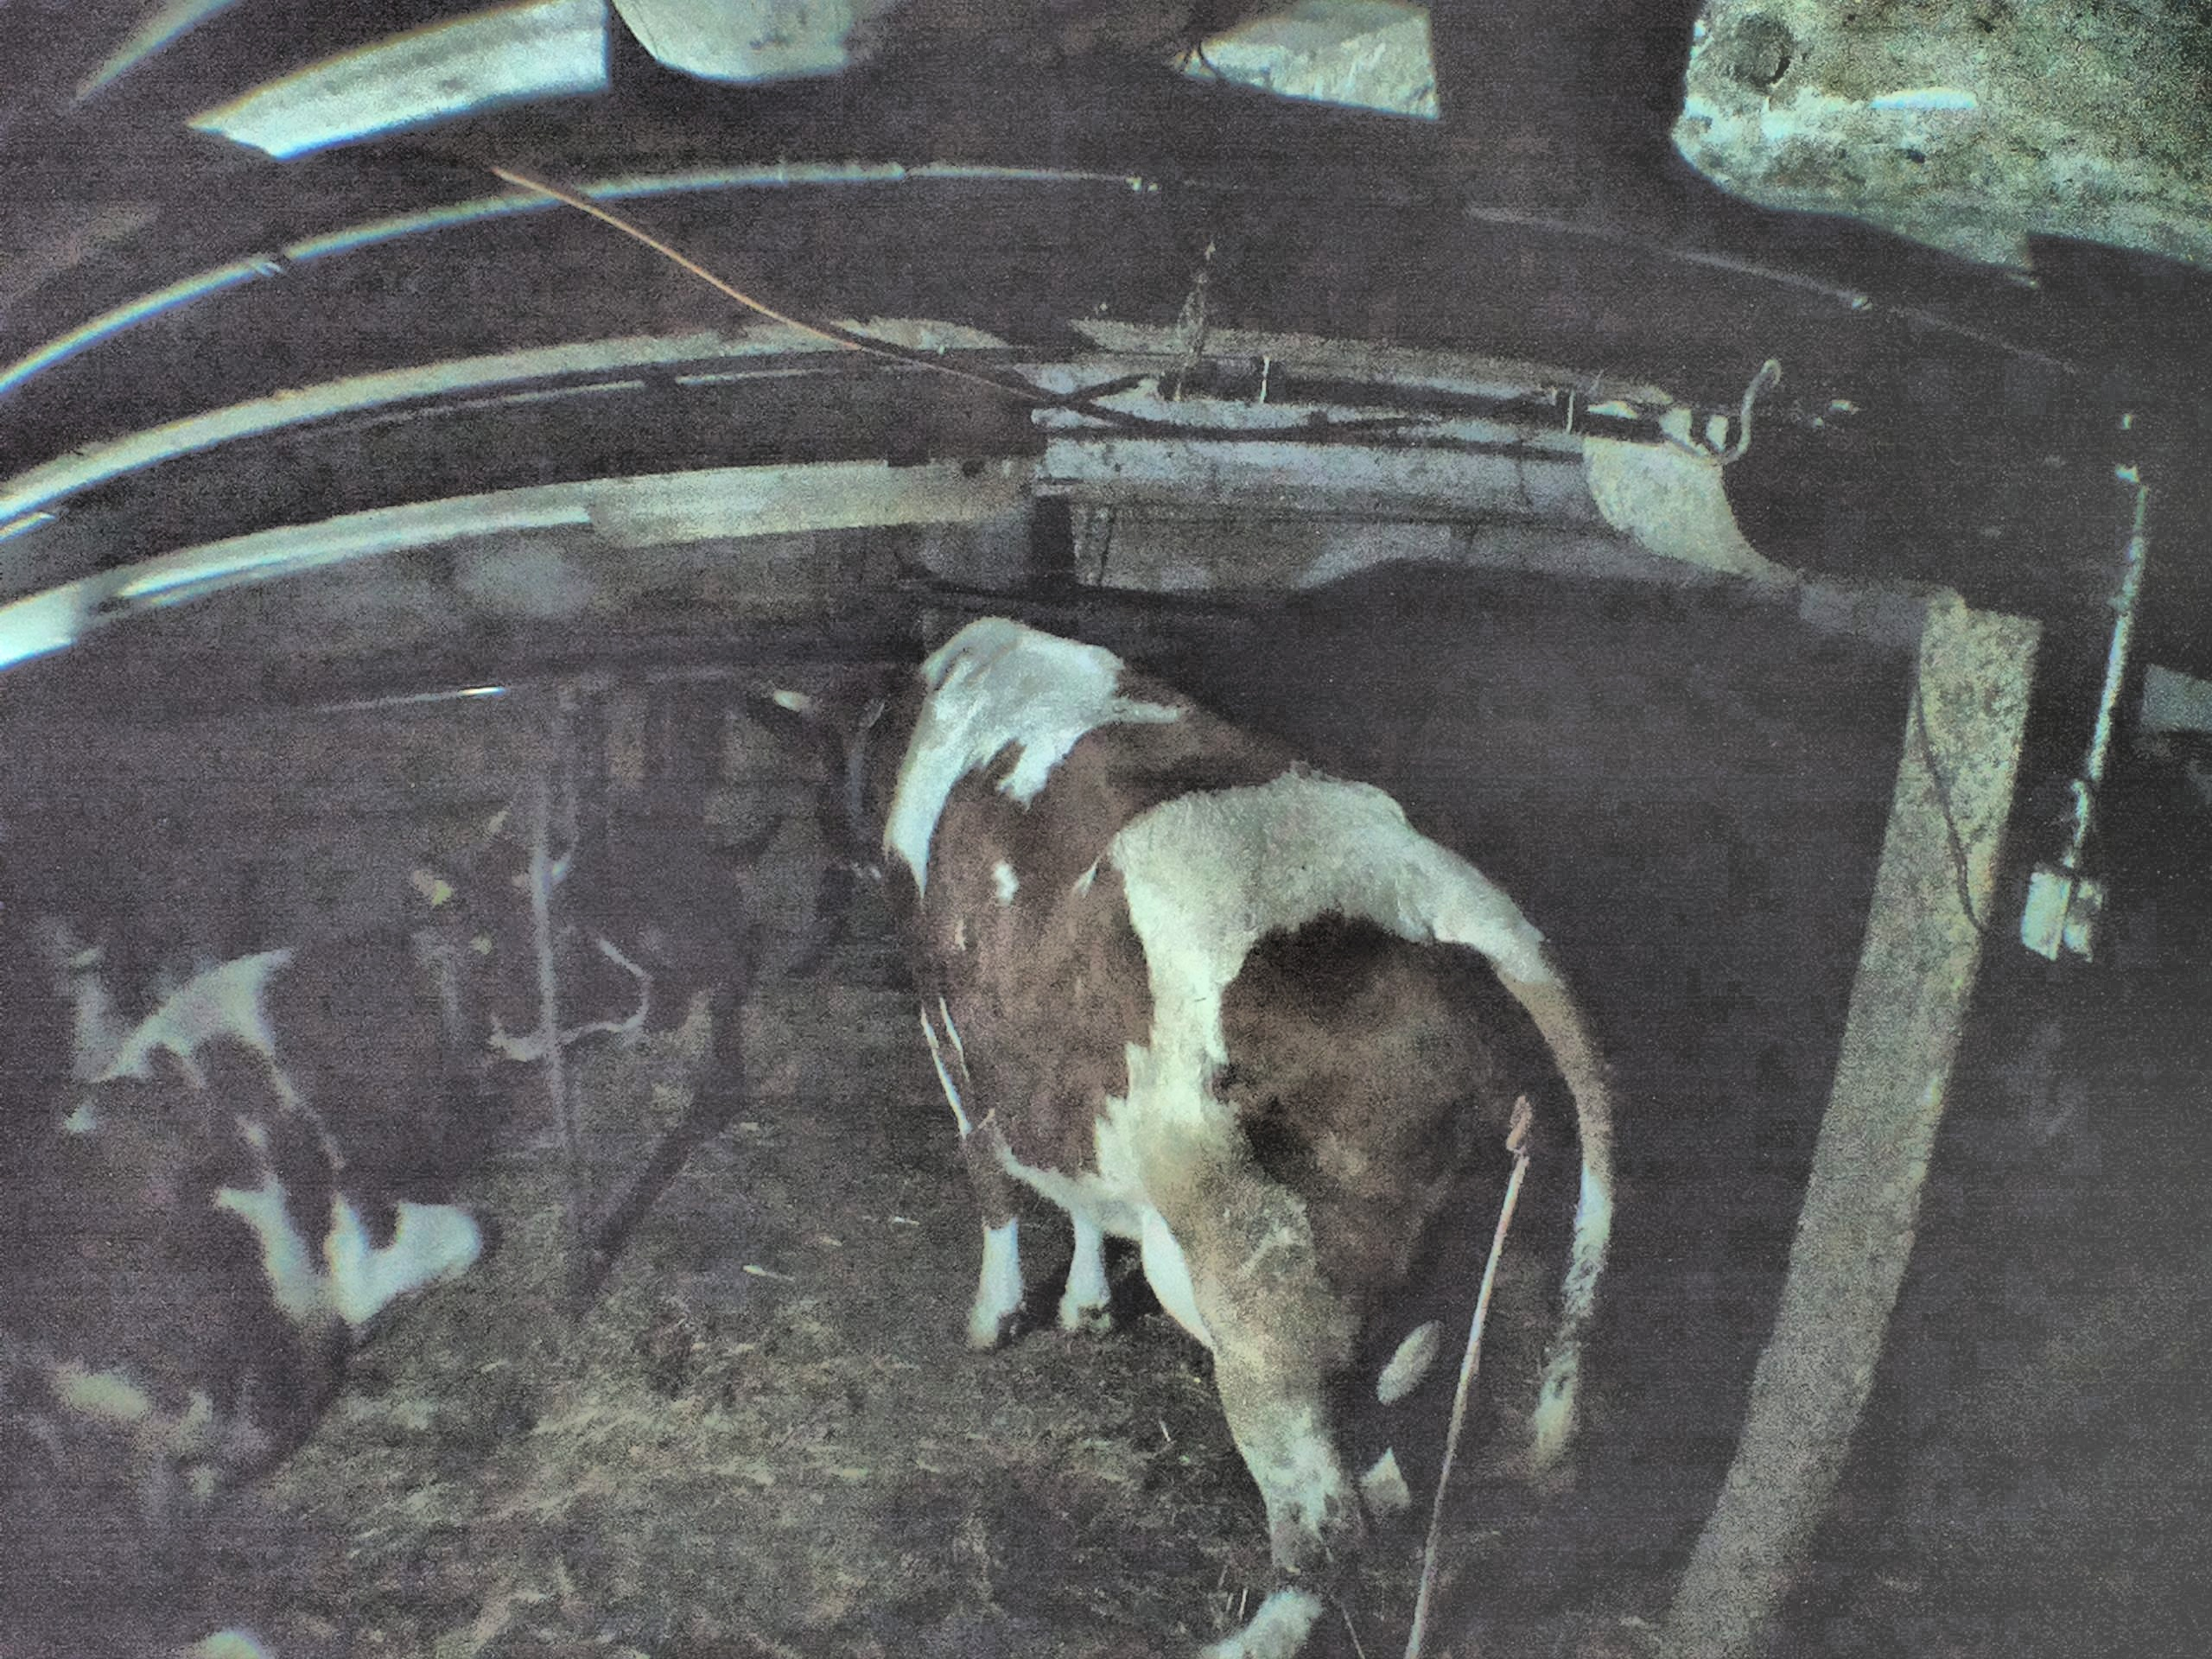
\includegraphics[scale=0.075]{Grafiken/schleim.jpg}
	\caption{Die Nachgeburt wird ausgelöst.} 
	\label{fig: Die Nachgeburt wird ausgelöst.}
\end{figure}